\chapter{Adaptive Ensemble Methods}
\label{ch:ensemblemethods}

%Advanced analysis of data streams is quickly becoming
%a key area of data mining research as the number of applications
%demanding such processing increases.
%Online mining when such data streams evolve over time,
%that is when concepts drift or change completely,
%is becoming one of the core issues.
%When tackling non-stationary concepts, ensembles of classifiers
%have several advantages over single classifier methods:
%they are easy to scale and parallelize, they can adapt to change
%quickly by pruning under-performing parts of the ensemble, and they
%therefore usually also generate more accurate concept descriptions.

Online mining when data streams evolve over time,
that is when concepts drift or change completely,
is becoming one of the core issues of advanced analysis of data streams.
When tackling non-stationary concepts, ensembles of classifiers
have several advantages over single classifier methods:
they are easy to scale and parallelize, they can adapt to change
quickly by pruning under-performing parts of the ensemble, and they
therefore usually also generate more accurate concept descriptions.
This chapter presents two new  variants of Bagging: \adwin
Bagging and Adaptive-Size Hoeffding Tree (ASHT) Bagging.

%Bagging and Boosting are two of the best known ensemble learning algorithms.
%\begin{itemize}
% \item Bootstrap Aggregating (bagging) generates multiple bootstrap training sets from the
%original training set and uses each of them to generate a classifier for inclusion in the
%ensemble. 
%\item A Boosting algorithm %is formally defined to be an algorithm that 
%converts a weak learning algorithm into a strong learning algorithm. That is, 
%it boosts a learning algorithm that performs slightly better than random chance
%on a problem into an algorithm that performs properly on that problem.
%The AdaBoost algorithm is the most popular boosting algorithm. It generates a
%sequence of base models with different weight distributions over the training set.
%\end{itemize}
\BEGINOMIT
In~\cite{oza01online} Oza and Russell developed online versions %ensemble learning algorithms
of bagging and boosting for Data Streams. They show how the process
of sampling bootstrap replicates from training data can be simulated in a 
data stream context. 
They observe that the probability that any individual
example will be chosen for a replicate %is governed by a Binomial distribution,
%so the sampling process can be approximated by considering each example
%in turn and randomly deciding with a Binomial probability distribution how
%many times to include the example in the formation of a replicate set. %The
%difficulty with this solution is that the number of examples needs to be
%known in advance. 
%Oza and Russell get around this by considering that the 
%Binomial distribution 
tends to a Poisson(1) distribution. 

For the boosting method, Oza and Russell 
note that the weighting procedure of AdaBoost actually divides the total example 
weight into two halves \--- half of the weight is assigned to the correctly
classified examples, and the other half goes to the misclassified examples. %As
%the ensemble gets more accurate the number of misclassified examples should
%progressively get less and less relative to the number of correct classifications.
%In turn, the misclassified set gets more weight per example than the correctly
%classified set. This motivates a weight update procedure that 
%is intended to simulate the batch weight behaviour in a streaming environment,
%much like the online bagging algorithm is designed to simulate the creation of
%bootstrap replicates. Once again 
They use the Poisson distribution for 
deciding the random probability that an example is used for training, only this time
the parameter changes according to the boosting weight of the example
as it is passed through each model in sequence.

Pelossof et al. presented in~\cite{OCBoost} Online Coordinate Boosting, a new
online boosting algorithm for adapting the weights of a boosted classifier, which
yields a closer approximation to Freund and Schapire's AdaBoost algorithm.
The weight update procedure is derived by minimizing AdaBoost's loss when viewed in an incremental
form. This boosting method may be reduced to a form similar to Oza and Russell's algorithm.
%not performing some corrections in their algorithm.}
 %If they do not perform some corrections in their algorithm, they reduce it 
%to a form similar to Oza and Russell's algorithm.
\ENDOMIT

\BEGINOMIT
Chu and Zaniolo proposed in~\cite{FLBoost} Fast and Light Boosting for adaptive mining
of data streams. It is based on a dynamic sample-weight assignment scheme that is extended
to handle concept drift via change detection. The change detection approach aims at 
significant data changes that could cause serious deterioration of the ensemble performance,
and replaces the obsolete ensemble with one built from scratch.
\ENDOMIT

\section{New method of Bagging using trees of different size}
\label{hast}

\begin{figure}
\begin{center}
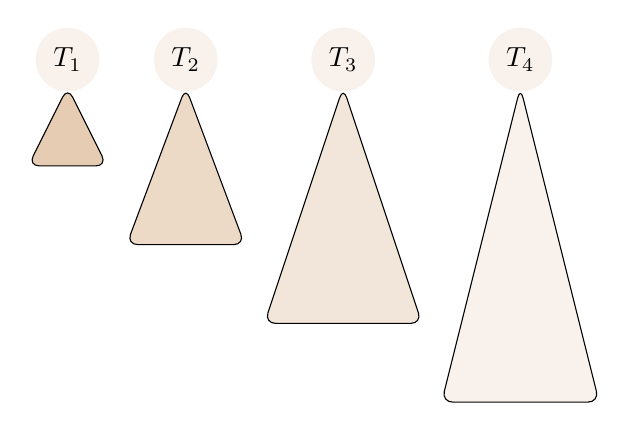
\begin{tikzpicture}
\node at (0.5cm,3.35cm) [circle,draw=brown!10,fill=brown!10] {$T_1$};
\node at (2cm,3.35cm) [circle,draw=brown!10,fill=brown!10] {$T_2$};
\node at (4cm,3.35cm) [circle,draw=brown!10,fill=brown!10] {$T_3$};
\node at (6.25cm,3.35cm) [circle,draw=brown!10,fill=brown!10] {$T_4$};
\draw[fill=brown!40,rounded corners] (0cm,2cm) -- (.5cm,3cm) -- (1cm,2cm) -- cycle;
\draw[fill=brown!30,rounded corners] (1.25cm,1cm) -- (2cm,3cm) -- (2.75cm,1cm) -- cycle;
\draw[fill=brown!20,rounded corners] (3cm,0cm) -- (4cm,3cm) -- (5cm,0cm) -- cycle;
\draw[fill=brown!10,rounded corners] (5.25cm,-1cm) -- (6.25cm,3cm) -- (7.25cm,-1cm) -- cycle;
\end{tikzpicture} 
\end{center}

\caption{An ensemble of trees of different size}
\label{fig:trees}
\end{figure}


\begin{figure}
\begin{center} 
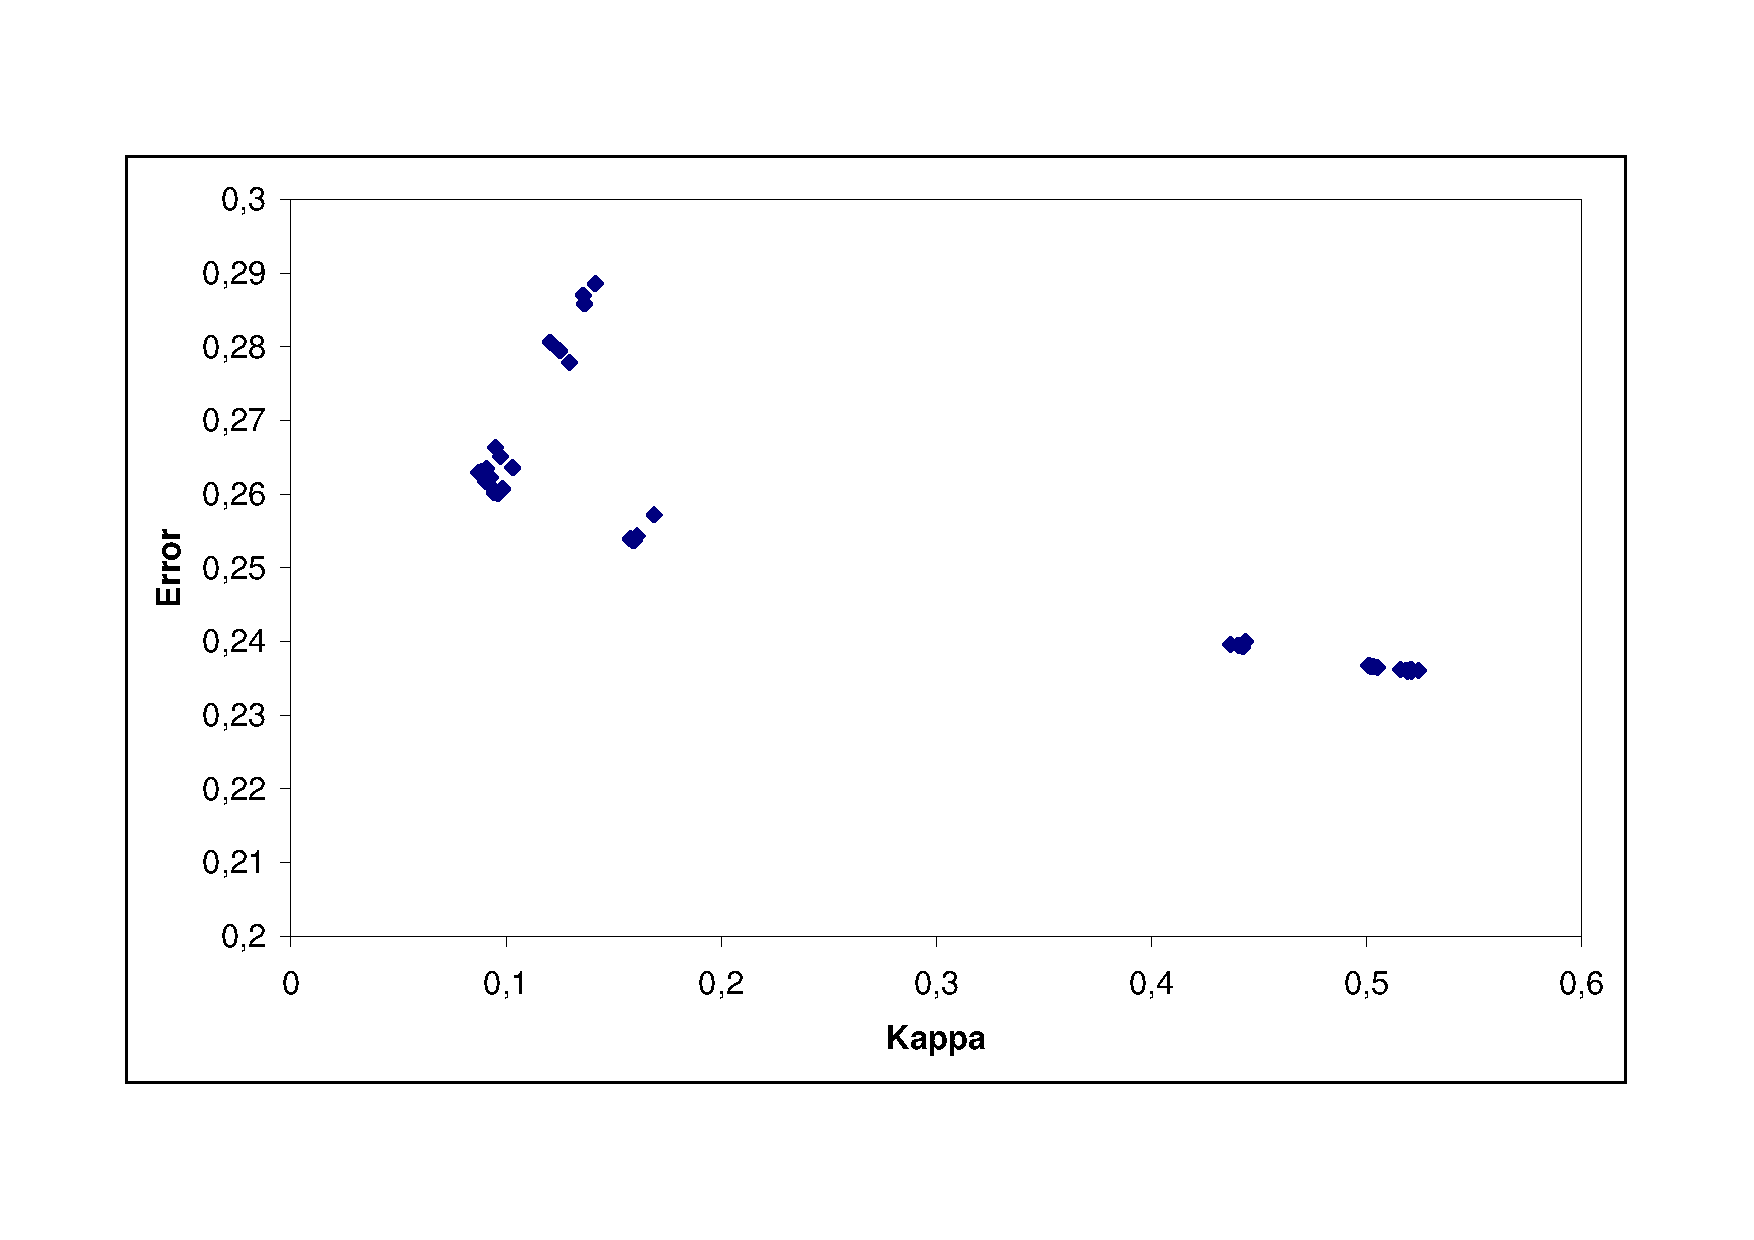
\epsfig{file=figures/Kappa1, scale=\sizeGraph} 
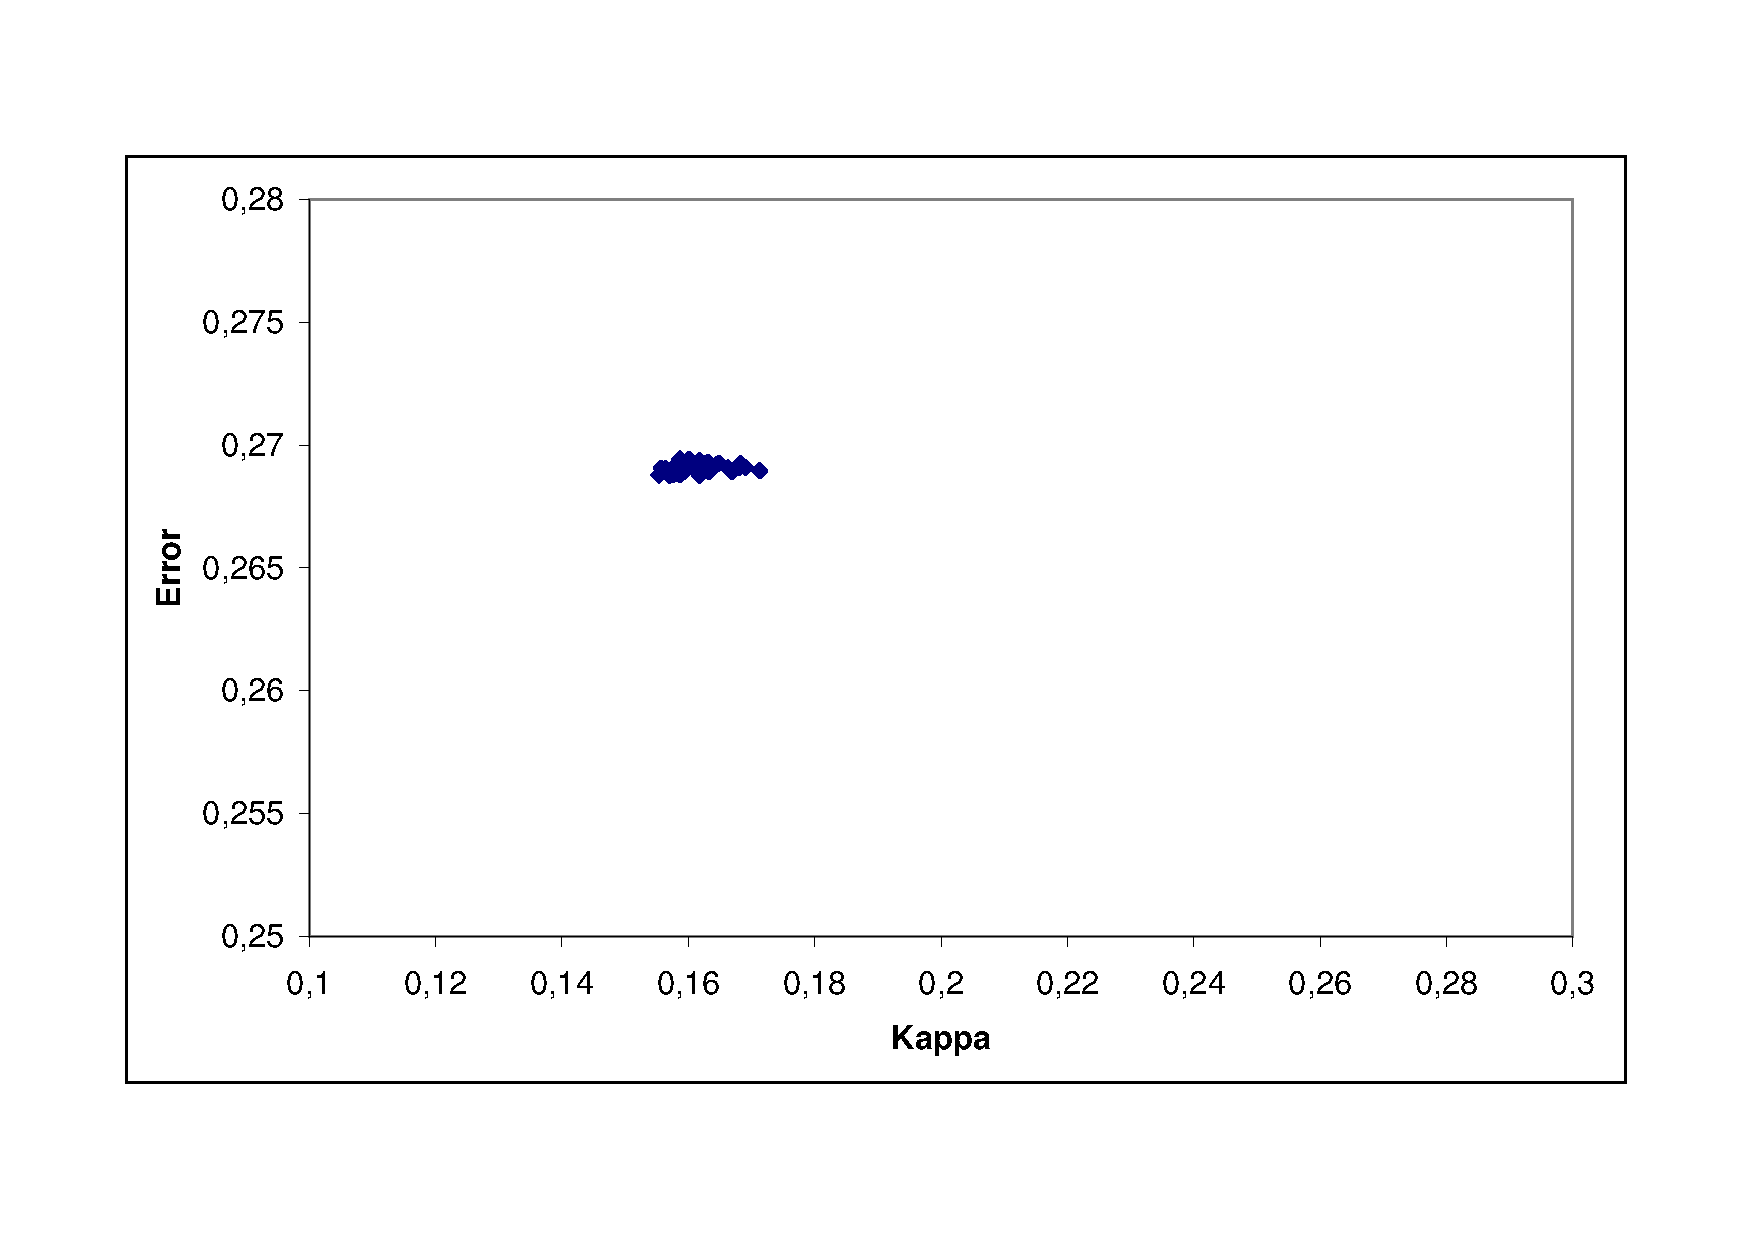
\epsfig{file=figures/Kappa2, scale=\sizeGraph} 

\end{center}
\caption{Kappa-Error diagrams for ASHT bagging (left) and bagging (right) on dataset RandomRBF with drift,
plotting 90 pairs of classifiers.}

\label{fig:kappa}
\end{figure}
\BEGINOMIT
In this section, we present a new method of bagging using Hoeffding Trees of different sizes.

A {\em Hoeffding tree}~\cite{vfdt} is an incremental, anytime decision tree 
induction algorithm that is capable of learning from massive data streams, 
assuming that the distribution generating examples does not change over time.
Hoeffding trees exploit the fact that a small sample can often be enough to choose 
an optimal splitting attribute. This idea is supported mathematically by the 
Hoeffding bound, which quantifies the number of observations (in our case, 
examples) needed to estimate some statistics within a prescribed precision (in 
our case, the goodness of an attribute). 
More precisely, the Hoeffding bound states that with probability $1 - \delta$, 
the true mean of a random variable of range $R$ will not differ from the estimated 
mean after $n$ independent observations by more than:
$$ \epsilon = \sqrt{\frac{R^2 \ln(1/\delta)}{2n}}.$$
A theoretically appealing feature of Hoeffding Trees not shared by other 
incremental decision tree learners is that it has sound guarantees of performance. 
Using the Hoeffding bound one can show that its output is asymptotically nearly 
identical to that of a non-incremental learner using infinitely many examples.
See \cite{vfdt} for details. 
\ENDOMIT
\BEGINOMIT
{\em Hoeffding Window Trees}~\cite{} are decision trees 
that using Hoeffding bounds, maintain a sliding window of instances, 
and that .

\begin{itemize}
 \item place one or more change detectors at every node that will
raise a hand whenever something worth attention happens at the node
 \item create, manage, switch and delete alternate trees
 \item maintain estimators of only relevant statistics at the nodes of the current sliding window
\end{itemize}

A {\em Hoeffding Adaptive Tree} is a decision tree that evolving from Hoeffding 
Window Tree, adaptively learn from data streams that change over time
without needing a fixed size of sliding window. The optimal size of the
sliding window is a very difficult parameter to guess for users, since it depends
on the rate of change of the distribution of the dataset.
The general idea is simple: we place instances of estimators of frequency
statistics at every node, that is, replacing each
counters in the Hoeffding Window Tree with an instance of an estimator.
\ENDOMIT

In this section, we introduce the Adaptive-Size Hoeffding Tree (ASHT). It is derived
from the Hoeffding Tree algorithm with the following differences:

\begin{itemize}
\item it has a maximum number of split nodes, or {\em size}
\item after one node splits, if the number of split nodes of the ASHT tree is higher than the
maximum value, then it deletes some nodes to reduce its size
\end{itemize}

The intuition behind this method is as follows: smaller trees adapt more quickly to changes,
and larger trees do better during periods with no or little change,
simply because they were built on more data.
Trees limited to size $s$ will be reset about twice as often as
trees with a size limit of $2s$.
This creates a set of different reset-speeds for an ensemble of such trees, and
therefore a subset of trees that are a good approximation for the current rate of change. 
It is important to note that resets will happen all the time, even for stationary datasets,
but this behaviour should not have a negative impact on the ensemble's predictive performance.

When the tree size exceeds
the maximun size value, there are two different delete options:
\begin{itemize}
 \item delete the oldest node, the root, and all of its children %delete oldest node, the root node and all its children
except the one where the split has
been made. After that, the root of the
child not deleted becomes the new root
delete the oldest node, the root, and all of its children.

 %\item delete worst error node: the node with higher error and its childs
 \item delete all the nodes of the tree, i.e., restart from a new root.
\end{itemize}



We present a new bagging method that uses these Adaptive-Size Hoeffding Trees
and that sets the size for each tree (Figure~\ref{fig:trees}). 
The maximum allowed size for the $n$-th ASHT tree is
twice the maximum allowed size for the $(n-1)$-th tree. Moreover, each tree
has a weight proportional to the inverse of the square of its error, and
%The size of ASHT 
%tree $n$ is two times the size of ASHT tree $n-1$. Moreover, it uses  a weight 
%proportional to the inverse of the square of the error, and 
it monitors its error
with an exponential weighted moving average (EWMA) with $\alpha=.01$. The size of the first tree is $2$. 

With this new method, we attempt to improve bagging performance by increasing tree diversity.
It has been observed that boosting tends to produce a more diverse set of classifiers
than bagging, and this has been cited as a factor in increased performance~\cite{MargineantuD97}.

We use the Kappa statistic $\kappa$ to show how using trees of different size, we increase
the diversity of the ensemble. 
Let's consider two classifiers $h_a$ and $h_b$, a data set containing $m$ examples, and
a contingency table where cell $C_{ij}$ contains the number of examples for which $h_a(x)=i$
and $h_b(x)=j$. If $h_a$ and $h_b$ are identical on the data set, then all non-zero counts 
will appear along the diagonal. If $h_a$ and $h_b$ are very different, then there should be
a large number of counts off the diagonal. We define
$$\Theta_1= \frac{\sum^{L}_{i=1} C_{ii}}{m}$$
$$\Theta_2 = \sum^L_{i=1} \left(  \sum^L_{j=1} \frac{C_{ij}}{m} \cdot \sum^L_{j=1}\frac{C_{ji}}{m} \right) $$
We could use $\Theta_1$ as a measure of agreement, but in problems where one class is much
more common than others, all classifiers will agree by chance, so all pair of classifiers
will obtain high values for $\Theta_1$. To correct this,
the $\kappa$ statistic is defined as follows:
$$ \kappa = \frac{\Theta_1 -\Theta_2}{1-\Theta_2}$$
$\kappa$ uses $\Theta_2$, the probability that two classifiers agree by chance, given the observed counts in the table.
% The $\kappa$ statistic is defined as follows:
If two classifiers agree on every example then $\kappa = 1 $, and if their predictions
coincide purely by chance, then $\kappa = 0$.



We use the Kappa-Error diagram to compare the diversity of normal bagging with bagging using trees
of different size. The Kappa-Error diagram is a scatterplot where each point corresponds to a pair
of classifiers. The $x$ coordinate of the pair is the $\kappa$ value for the two classifiers. 
The $y$ coordinate is the average of the error rates of the two classifiers.

Figure~\ref{fig:kappa} shows the Kappa-Error diagram for the Random RBF dataset with drift parameter or
change speed equal to 0.001.% speed of change of $.001$. 
We observe that bagging classifiers are 
very similar to one another and that the decision tree classifiers of different size are very diferent from
one another.

\section{New method of Bagging using \adwin}% and Boosting}
\label{adwinbagging}
%\BEGINOMIT
\adwinb\cite{bif-gav}, as seen in Chapter~\ref{ch:adwin} is a change detector and estimator that solves in a 
well-specified way the problem of tracking the average of a stream of bits or 
real-valued numbers. \adwin keeps a variable-length window of recently seen 
items, with the property that the window has the maximal length statistically 
consistent with the hypothesis ``there has been no change in the average value
inside the window". 

%\BEGINOMIT
More precisely, an older fragment of the window is dropped if and only if 
there is enough evidence that its average value differs from that of 
the rest of the window. 
This has two consequences: one, that change reliably declared whenever
the window shrinks; and two, that at any time the average over the existing
window can be reliably taken as an estimation of the current average in the stream
(barring a very small or very recent change that is still not statistically 
visible). %A formal and quantitative statement of these two points (a theorem)
%appears in \cite{bif-gav}. 
%\ENDOMIT

\adwin is parameter- and assumption-free in the sense that 
it automatically detects and adapts to the current rate of change. 
Its only parameter is a confidence bound $\delta$,
indicating how confident we want to be in the algorithm's output, 
inherent to all algorithms dealing with random processes. 

Also important for our purposes, \adwin does not maintain the window
explicitly, but compresses it using a variant of the exponential histogram
technique in \cite{babcock-sampling}. This means that it keeps a window of length $W$
using only $O(\log W)$ memory and $O(\log W)$ processing time per item, 
rather than the $O(W)$ one expects from a na{\"\i}ve implementation. 
%\ENDOMIT

\adwin Bagging is the online bagging method % and boosting algorithms 
implemented in MOA with the  addition of the \adwin algorithm as a change 
detector and as an estimator for the weights of the boosting method.
When a change is detected, the worst classifier of the ensemble of classifiers 
is removed and a new classifier is added to the ensemble.

\section{Adaptive Hoeffding Option Trees}
\label{Ssadahot}
                                                                  
{\em Hoeffding Option Trees}~\cite{optiontrees} 
explained in Section~\ref{sec:hot} are regular Hoeffding trees 
containing additional option nodes that allow several tests to be applied, 
leading to multiple Hoeffding trees as separate paths. 
%  Hoeffding Option Trees 
They consist of a single structure that efficiently represents multiple
trees. A particular example can travel down multiple paths of the tree, contributing, 
in different ways, to different options.
% The class of a test example is
%determined by a committee made up of the predictions of all leaf nodes reached.
%In the context of a data stream, the idea is to grow multiple options in the same
%manner as a single Hoeffding tree. By doing so the effects of limited lookahead
%and instability are mitigated, leading to a more accurate model.

An {\em Adaptive Hoeffding Option Tree} is a Hoeffding Option Tree with the following improvement:
each leaf stores an estimation of the current error. It uses an EWMA
estimator with $\alpha =.2$.
The weight of each node in the voting process is 
proportional to the square of the inverse of the error.

\section{Method performance}

Bagging is clearly the best method in terms of accuracy. This superior position
is, however, achieved at high cost in terms of memory and time. 
\adwin Bagging and ASHT Bagging are the most accurate methods for most datasets, but they 
are slow.
%have a low prediction speed.
 \adwin Bagging is slower than ASHT Bagging and for some datasets it 
needs more memory. 
ASHT Bagging using weighted classifiers and replacing oversized trees 
with new ones seems to be the most accurate ASHT bagging method.
We observe that bagging using 5 trees of different size may be 
sufficient, as its error is not much {higher} %%%lower 
than for 10 trees, but it is nearly {twice as fast}. %%two times faster.
Also Hoeffding trees using drift detection methods are faster but less accurate methods.

 In~\cite{optiontrees}, a range of option limits were tested and averaged across all datasets without
concept drift to determine the optimal number of paths. This optimal number of options was five.
Dealing with concept drift, we observe that increasing the number of options to 50, 
 a significant improvement is obtained in accuracy for some datasets. 
